\documentclass[Letter,11pt]{article}
\usepackage{url}
\usepackage[utf8x]{inputenc}
\usepackage{amsmath}
\usepackage{graphicx}
\usepackage[margin=1in]{geometry}
\graphicspath{{Pictures/}}
\usepackage[colorinlistoftodos]{todonotes}
\usepackage{listings}
\usepackage[american voltages, americancurrents,siunitx]{circuitikz}
\usepackage{pgfgantt}
\usepackage{lscape}
\usepackage{tikz-er2}
\usepackage{fast-diagram}
\usepackage{tikz}
\usepackage{multirow}
\usepackage{xcolor,colortbl}
\usepackage{array}
\usepackage{hhline}
\usepackage{helvet}
\renewcommand{\familydefault}{\sfdefault}
\usetikzlibrary{shapes.geometric,arrows,automata,calc,shapes, positioning}


\newcommand{\labs}{\renewcommand{\chaptername}{Lab}}
\newcommand{\Appendix}{	\makeatletter 
					\appendix
					\renewcommand\chaptername{Appendix}}

\NewDocumentCommand{\rot}{O{45} O{1em} m}{\makebox[#2][l]{\rotatebox{#1}{#3}}}%
\newcolumntype{M}{>{\centering\arraybackslash}m}

\lstset{language=C,
	numbers=left,
	keywordstyle=\color{kewordPurple},
	stringstyle=\color{stringBlue},
	commentstyle=\color{comentGreen},
	morecomment=[l][\color{magenta}]{\#}}

%
% colors
%
\definecolor{kewordPurple}{RGB}{127,0,85}
\definecolor{comentGreen}{RGB}{63,127,95}
\definecolor{stringBlue}{RGB}{42,0,255}
%http://brand.msu.edu/design-visual/index.html
\definecolor{MSUgreen}{RGB}{23,69,59}
\definecolor{othergreen}{RGB}{13,177,75}
\definecolor{MSUgray}{RGB}{153,162,162}
\definecolor{MSUorange}{RGB}{240,133,33}
\definecolor{MSUgreenBlue}{RGB}{0,129,131}
\definecolor{MSUgreenBlue}{RGB}{0,129,131}
\definecolor{MSUBlueGray}{RGB}{144,154,183}
\definecolor{MSUDarkGray}{RGB}{83,80,84}
\definecolor{MSULimeGreen}{RGB}{209,222,63}
\definecolor{MSUTan}{RGB}{232,217,181}
\definecolor{MSUTanDark}{RGB}{200,154,88}
\definecolor{MSUOffGreen}{RGB}{148,174,74}
\definecolor{MSUPurple}{RGB}{110,0,95}
\definecolor{MSUDarkorange}{RGB}{203,90,40}



\begin{document}
	%make the tile
	%%%%%%%%%%%%%%%%%%%%%%%%%%%%%%%%%%%%%%%%%
% University Assignment Title Page 
% LaTeX Template
% Version 1.0 (27/12/12)
%
% This template has been downloaded from:
% http://www.LaTeXTemplates.com
%
% Original author:
% WikiBooks (http://en.wikibooks.org/wiki/LaTeX/Title_Creation)
%
% License:
% CC BY-NC-SA 3.0 (http://creativecommons.org/licenses/by-nc-sa/3.0/)
% 
% Instructions for using this template:
% This title page is capable of being compiled as is. This is not useful for 
% including it in another document. To do this, you have two options: 
%
% 1) Copy/paste everything between \begin{document} and \end{document} 
% starting at \begin{titlepage} and paste this into another LaTeX file where you 
% want your title page.
% OR
% 2) Remove everything outside the \begin{titlepage} and \end{titlepage} and 
% move this file to the same directory as the LaTeX file you wish to add it to. 
% Then add \input{./title_page_1.tex} to your LaTeX file where you want your
% title page.
%
%%%%%%%%%%%%%%%%%%%%%%%%%%%%%%%%%%%%%%%%%
	
\begin{titlepage}
		             
		\newcommand{\HRule}{\rule{\linewidth}{0.5mm}} % Defines a new command for the horizontal lines, change thickness here
		
		\center % Center everything on the page
		
		%----------------------------------------------------------------------------------------
		%	HEADING SECTIONS
		%----------------------------------------------------------------------------------------
		
		\textsc{\LARGE Michigan State University}\\[0.5cm] % Name of your university/college
		\textsc{\Large Department Of Electrical and Computer Engineering}\\[0.5cm] % Major heading such as course name
		%\textsc{\large smaller big text}\\[0.5cm] % Minor heading such as course title
		\textsc{\Large ECE 480 Senior Design}\\[0.5cm]
		
		%----------------------------------------------------------------------------------------
		%	TITLE SECTION
		%----------------------------------------------------------------------------------------
		
		\HRule \\[0.2cm]
		{ \huge \bfseries Final Project Proposal\\ ArcelorMittal USA\\ Safety Equipment Bar Code Scanner}\\[0.2cm] % Title of your document
		\HRule \\[1.5cm]
		
		%----------------------------------------------------------------------------------------
		%	AUTHOR SECTION
		%----------------------------------------------------------------------------------------
		\noindent
		\begin{minipage}[t]{0.3\textwidth}
			\begin{flushleft} \large
				\emph{Team Members:}\\
				Kyle \textsc{Inch}\\
				Alexandria \textsc{Marone}\\
				Seth \textsc{McKisson}\\
				Trevor \textsc{Sabo}\\
				Ian \textsc{Grosh}\\ % Your name
			\end{flushleft}
		\end{minipage}% A new line will break it so dont Ian!
		\begin{minipage}{0.3\textwidth}
			\centering
			{\LARGE Design Team 3}
		\end{minipage}
		\begin{minipage}[t]{0.3\textwidth}
			\begin{flushright} \large
				\emph{Facilitator:}\\  % Supervisor's Name
				%\centering
				Dr. Bingsen \textsc{Wang}
				
			\end{flushright}
			
		\end{minipage}\\[1cm]
		
		% If you don't want a supervisor, uncomment the two lines below and remove the section above
		%\Large \emph{Author:}\\
		%John \textsc{Smith}\\[3cm] % Your name
		
		%----------------------------------------------------------------------------------------
		%	DATE SECTION
		%----------------------------------------------------------------------------------------
		
		{\large \today}\\[0.5cm] % Date, change the \today to a set date if you want to be precise
		
		%----------------------------------------------------------------------------------------
		%	LOGO SECTION
		%----------------------------------------------------------------------------------------
		
		
		
		\begin{minipage}[t]{0.4\textwidth}
			\begin{center} 
			
\includegraphics{egr_logo.png}%\\[1cm]  % Include a department/university logo - this will require the graphicx package
			\end{center}
		\end{minipage}%
		\begin{minipage}[t]{0.4\textwidth}
			\begin{center} 
		
\includegraphics{MSUSealBlack1inch.png}
			\end{center}
		\end{minipage}\\[2cm]
	\begin{abstract}
		Design team three has been asked to create a system to keep track of safety equipment on ArcelorMittal's buildings. To do this the team needs to build some systems. These systems will enable administrators to both monitor compliance standards on areas they are in charge of, and make sure that safety equipment is being properly checked and documented. Reports will be sent out periodically on the above to said administrators.  On the user end, an Android application  that uses a scanner will be created that will enable users to quickly answer questions on safety equipment standards.

	\end{abstract}
		%\\[1cm] 
		% Include a department/university logo - this will require the graphicx package
		%----------------------------------------------------------------------------------------
		


		
		
		%\vfill % Fill the rest of the page with whitespace
		
\end{titlepage}

			\tableofcontents
			\listoffigures
			\begingroup
			\let\clearpage\relax
			\listoftables
			\endgroup
			\newpage


\part{Overview of Customer's Requirements}
\section{Background Research}\label{research}
	There is background research that needs to be implemented to characterize primary hardware and software components that are needed for a successful project. \\
	\subsection{Assessing Customer Needs}

	The customer's needs, as well as the needs of their users, are team three's highest priority. Team three's sponsor, our primary point of contact, is Jim Lang with ArcelorMittal. Our sponsor clearly defines ArcelorMittal's needs, and how the user will be interacting with the system. Team three's customer's needs are clearly documented by ArcelorMittal. This documentation assess the needs and interests of the ultimate user. \\ 


	\subsection{Design Constraints}
	With customer needs comes design constraints. The first design constraint is time. Team three has been given one semester to deliver a complete solution. Another constraint is cost. Team three has been given a budget of \$500 to create this system.\\


	\subsection{Feasibility of Designs}
	Criteria to judge the feasibility of the design has been outlined by team three's sponsor ArcelorMittal. Team three was given requirements necessary for designing and implementing a Minimum Viable Product. The requirements are based on ArcelorMittal's current implementation of problem, Field ID. To satisfy necessary criteria, team three's goal is to implement a software-based solution, hence; automating the entire process. Ultimately feasibility will be judged based on universal usability. In order to rank the feasible designs, team three must also consider criteria based on speed of response time, organization of documentation, report generation, and ability to publish software development environment into production. \\
	Each set of conceptual designs/variations meets the feasibility criteria. Team three's solution meets the goals of the customer's needs; the proposed solution has been approved by both team sponsor and facilitator. Trade off studies that need be conducted to assess the above concerns are speed of response time, and difficulty to move team three's software development environment to production. In a software environment, feasible conceptual designs are always subjected to change. \\
	\subsection{Risks}
	A majority of risks revolve around the security of team three's proposed system. This is solved by the implementation and integration on ArcelorMittal's servers. Due to safety and liability restrictions, team three is unable to gain access to ArcelorMittal systems; most specifically their database. Team three's solution is designed to integrated into ArcelorMittal's existing system. \\
	\subsection{Overview of System Models}
	As the nature of this project is more software oriented then hardware, developing models for system senors, actuators, interfaces or other principle level system components are not a concern. As a result, no validation is needed. Similarly, issues involving control processes are not a concern. \\
	However, Operating Systems at different interconnections distances is a concern. ArcelorMittal has a special requirement that team three's mobile application must operate without WIFI; this issue must be accommodated. Additionally storage on the Nexus 7 tablet is also a concern. A limit of 16GB of memory is crucial; therefore, team three's application must be well within that limit.  Finally, the software must be compatible with hardware specifics of the Nexus 7, which are a ULP GeForce graphics card, Quad Core processors, and 1GB of RAM \cite{nexus7}. \\
	
	\subsection{Developmental Strategy}
	Team three has picked a bottom-up approach. Team three will implement lower levels specifics at highest level of importance. This gives the team the ability to test database communication first. Further, when fusing data into the user interface, the API's implemented create connections for testing. This allows the team to efficiently design an experience while minimizing on constraints. Developmental tools for the environments will also be utilized for testing. \\ 

\section{High Level Languages}\label{highlevel}
	\subsection{Languages}
	As for compilers on the Back End most things will be written in the programming language Python, which does not have a compiler. For the email service, SMTP python libraries will be used, as well as various web framework libraries. The web framework libraries are provided by Django, a high-level Python Web framework. \\
	Android Application Development is written in Java which does have a compiler. On the administrator side, jQuery, Twitter's Bootstrap, will be used for web development.  A detailed implementation can be found in section \ref{WEBAPP}.  \\ 


\part{Technical}
\section{Project Definition}\label{def}
	This team has been assigned an industry sponsored project from ArcelorMittal, who need a way to track their industrial safety equipment within their buildings. In order to build the specified system team three will need to build three primary systems. The first being an Android application for operators to scan barcodes on safety locations and equipment. A web application to allow administrators to specify questions for specific pieces of safety equipment, and furthermore assign responsibility to workers. Finally, a server infrastructure will be created to ensure data is held properly and securely, host the web application, connect to the Android application, and generate reports. 
			
	\begin{figure}[h]
		\centering
		%%%%%%%%%%%%%%%%%%%%%%%%%%%%%%%%%%%
% System level conection diagram
%%%%%%%%%%%%%%%%%%%%%%%%%%%%%%%%%%%
\scalebox{.5}{
\begin{tikzpicture}[node distance=2cm]
	
	\tikzstyle{every node} = [ellipse, minimum width=3cm, minimum height=2cm,text centered, draw=black]
	\tikzstyle{arrow} = [thick,->]
	%\tikzstyle{arrow} = [->, >=latex', shorten >=1pt, thick]
	
	\node (fram) {Web Framework};
	\node (app) [above left=1cm and 3cm of fram] {Mobble Aplication};
	\node (web) [above=of fram] {Web Aplication};
	\node (email) [above right=1cm and 3cm of fram] {Emails \& Reports};
	\node (db) [below=of fram] {Databace};
	
	%\path[every node/.style={font=\sffamily}]
	%  (fram) edge[bend right=10] node  {Get}  (app)
	%  (app) edge[bend right=10] node  {Save}  (fram)
	%  (web) edge[bend right=10] node {Get}  (fram)
	%  (fram) edge[bend right=10] node {}  (web)
	%  (email) edge[bend right=10] node {}  (fram)
	%  (fram) edge[bend right=10] node {}  (email)
	%  (fram) edge node {} (db);
	\draw [bend left] (app) -- (fram)
    %\draw (fram) arc -- (app);
	%\draw (app) arc -- (fram);
	%\draw [arrow] (fram) -- (app);
	%\draw [arrow,bend left=45] (app) -- (fram);
	%\draw [arrow] (fram) -- (web);
	%\draw [arrow] (fram) -- (email);
	%\draw [arrow,bend right] (fram) -- (db);
	
	
	
\end{tikzpicture}
}

%\draw [arrow] (start) -- (in1);
%\draw [arrow] (dec1) -- node {yes} (pro2a);
%\draw [arrow] (dec1) -- node[anchor=south] {no} (pro2b);

		\caption{\label{sysConn} System Components}
	\end{figure}
	
	\subsection{Scope}\label{scope}
	In order to guide the teams design project and ensure the project has limits of what the team will build, a project scope has been defined:
	\\
	\begin{minipage}[t]{0.5\textwidth}
		\begin{itemize}
			\item \textbf{Mobile Application}
			\begin{itemize}
				\item Off-line mode
				\item Barcode scanning
				\item Barcode based questions
			\end{itemize}
			\item \textbf{Sever side Database and middle-ware}
			\begin{itemize}
				\item Host:
					\subitem Web application
					\subitem Database API for mobile application
			\end{itemize}
			\item\textbf{ Emails \& Reports}
			\begin{itemize}
				\item Inform administrators of:
					\subitem Failing devices
					\subitem Delinquent inspectors
				\item Inform inspectors of:
					\subitem Upcoming inspections
					\subitem Missed inspections
			\end{itemize}
		\end{itemize}
	\end{minipage}
	\begin{minipage}[t]{0.5\textwidth}
		\begin{itemize}
			\item \textbf{Web Application}
				\begin{itemize}
					\item Add locations to the database
					\item Add safety equipment types to the database
					\item Create questions
					\item Associate barcodes with:
						\subitem Locations
						\subitem Safety equipment
					\item Associate locations with:
						\subitem Safety equipment
						\subitem Questions
					\item Associate safety equipment with
						\subitem Locations
						\subitem Questions
					\item Add questions to reports
					\item Create timetable for reports
					\item Add recipient to reports
				\end{itemize}
		\end{itemize}
	\end{minipage}
		
	\subsection{Function Definition} 
		In order to justify the existence of items in Part~\ref{scope} the team created a number of function definitions. These definitions were then consolidated into the FAST diagram in Figure~\ref{fast1} along with a more detailed description.
		\begin{figure}[h]
			\centering
			%%%%%%%%%%%%%%%%%%%
%Fast Diogram
%%%%%%%%%%%%%%%%%%%

\begin{fast}{Ensure Compliance}
	\fastFT{Verify Standards}{
		\fastFT{Set Requirements}{}
		\fastFT{Set Responsibility}{}
		\fastFT{Schedule Checklist}{}
	}
	\fastFT{Keep Records}{
		\fastFT{Collect Data}{}
		\fastFT{Generate Reports}{}
	}
	\fastFT{Recognize Failures}{}	
\end{fast}

			\caption{\label{fast1} FAST Digram}
		\end{figure}
		The Primary function for the project is \textbf{Ensure Compliance} This is the main goal of the system we have been commissioned to build. From our primary function are derived two secondary functions each having there own tertiary functions:
		\begin{itemize}
			\item Verify Standards:\\
			In order to ensure compliance with all pertinent safety regulations the system must be able to check the and verify that all the stranded are being upheld in the various locations and across the numerous safety devices.
			\item Keep Records:\\
			In order to ensure that all of the safety laws and regulations are followed the team must keep records of all the locations which must have safety equipment present in a building, what safety equipment must be present, and how to verify that it is in working condition.  

			\item Recognize Failures:\\
			In order to recognize failures, the team needs to recognize when a piece of safety equipment is not in compliance. This could mean a variety of things, the equipment could not pass the safety inspections, or the equipment could not be present.   

		\end{itemize}
		From the secondary function Keep Records the team has derived: 
		\begin{itemize}
			\item Generate Reports:\\
			In order to keep records and ensure that every location and item is in compliance the system must be able to generate reports on any set of data on which record are kept. 
		\end{itemize}
		From the secondary function Verify Standards the team has derived:
		\begin{itemize}
			\item Set Requirements:\\
			In order to verify standards the system must be able to set complacence requirements for each location and item which is being tracked by the system.
			\item Set Responsibility:\\
			The standards are being upheld a person must be assigned Responsibility for a number of locations and items within the system. Once this Responsibility is set the owner can be held accountably for there set of locations and items. 
			\item Schedule Checklists:\\
			So that standards are verified  checklists should be generated to show those who are responsible for items which items need to be checked to ensure compliance.
		\end{itemize}
		
	\subsection{Use example}
		Here the team will use the data from the project description provided an example of how the team plans the how the system will be used.
		  
		%\begin{figure}
			%\centering
			%%%%%%%%%%%%%%%%%
% flow 1
%%%%%%%%%%%%%%%%
\scalebox{.5}{
	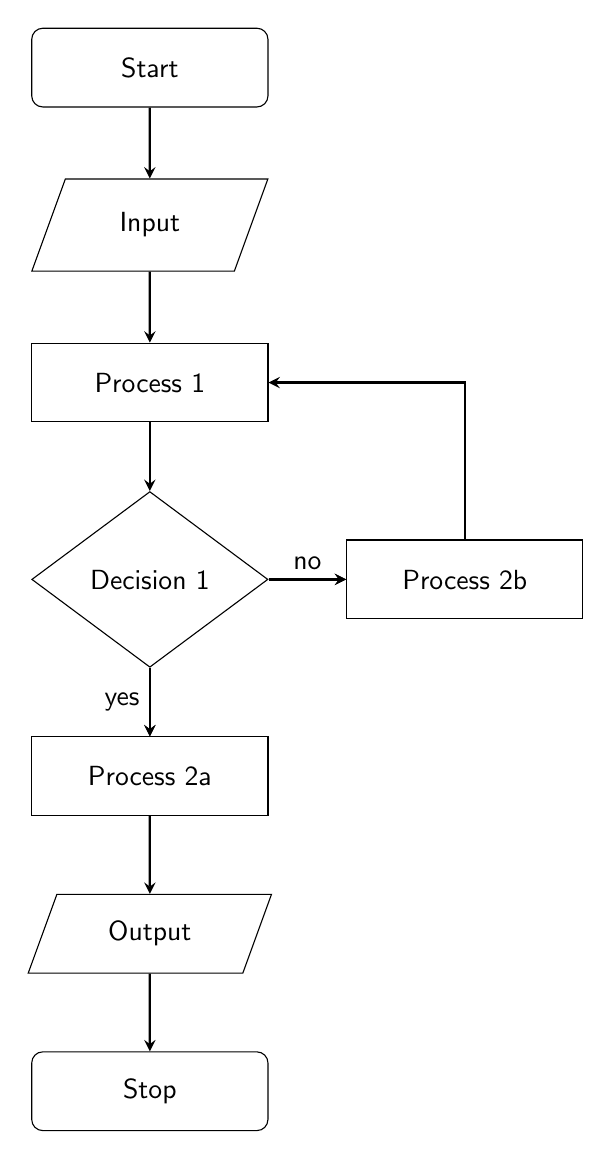
\begin{tikzpicture}[node distance=2cm]
	\tikzstyle{startstop} = [rectangle, rounded corners, minimum width=3cm, minimum height=1cm,text centered, draw=black]
	\tikzstyle{process} = [rectangle, minimum width=3cm, minimum height=1cm, text centered, draw=black]
	\tikzstyle{decision} = [diamond, minimum width=3cm, minimum height=1cm, text centered, draw=black]
	\tikzstyle{io} = [trapezium, trapezium left angle=70, trapezium right angle=110, minimum width=3cm, minimum height=1cm, text centered, draw=black]
	\tikzstyle{arrow} = [thick,->,>=stealth]
	
	\node (start) [startstop] {Start};
	\node (in1) [io, below of=start] {Input};
	\node (pro1) [process, below of=in1] {Process 1};
	\node (dec1) [decision, below of=pro1, yshift=-0.5cm] {Decision 1};
	\node (pro2a) [process, below of=dec1, yshift=-0.5cm] {Process 2a};
	\node (pro2b) [process, right of=dec1, xshift=2cm] {Process 2b};
	\node (out1) [io, below of=pro2a] {Output};
	\node (stop) [startstop, below of=out1] {Stop};
	
	\draw [arrow] (start) -- (in1);
	\draw [arrow] (in1) -- (pro1);
	\draw [arrow] (pro1) -- (dec1);
	\draw [arrow] (dec1) -- (pro2a);
	\draw [arrow] (dec1) -- (pro2b);
	%\draw [arrow] (dec1) -- node {yes} (pro2a);
	%\draw [arrow] (dec1) -- node {no} (pro2b);
	\draw [arrow] (dec1) -- node[anchor=east] {yes} (pro2a);
	\draw [arrow] (dec1) -- node[anchor=south] {no} (pro2b);
	\draw [arrow] (pro2b) |- (pro1);
	\draw [arrow] (pro2a) -- (out1);
	\draw [arrow] (out1) -- (stop);
	
	\end{tikzpicture}
}
			%\caption{\label{flow1} Database entity relations Diagram}
		%\end{figure}

		


\section{Technical Design}

	\subsection{Mobile Application}
	Design team three will build a mobile application for a tablet device which will allow a user to: download a database of safety equipment and locations to the mobile device to allow the user to operate with out access to the internet, scan barcodes of locations and safety devices to allow the user to answer a series of pass fail inspection questions, push question responses back to the database over the sponsor's internet. This last data push to the database will be completed when the user gets back to their desk, where there is WIFI available.
	\subsubsection{Mobile User Interface \& Experience}
	Design team three will create a user interface and experience (UI/UX) to guide the safety inspector through the process of an inspection. In  Figure~\ref{fig:login}, the user is prompted to login so that the data relevant to that user can be synced to the mobile device. By doing so that the inspection results can be recorded under the correct employee's name. \\
	If the user's device is connected to the internet, they will press the button labeled sync Figure~\ref{fig:splash} which will retrieve the inspection locations and safety device information pertinent to the user.
	Once the inspector reaches a location they will press the Scan Barcode Location button shown in Figure~\ref{fig:splash}.
	\begin{figure}[h]

		\begin{minipage}{0.5\textwidth}
			\centering
			
\includegraphics{StartPage.png}
			\caption{\label{fig:login}Mock up of Start Screen}
		\end{minipage}%real title space need to be here?
		\begin{minipage}{0.5\textwidth}
			\centering
			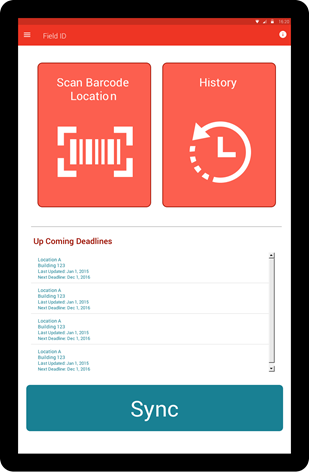
\includegraphics{SplashPage.png}
			\caption{\label{fig:splash}Mock up of splash screen}
		\end{minipage}
	\end{figure}

	\subsubsection{Barcode Scanning}
	The user will scan the barcode with the Android Application created. After successful scan, questions will pop up that need to be answered. On the event of a non-successful scan, a manual barcode insertion will be needed. The barcode scanning is done with a ZXing library (Zebra Crossing), and is open source and very well documented. Through testing we have found that this library produces a very reliable, accurate scanner and is perfect for the design specifications.\\
	In comparison, the Google Barcode  image recognition software was not quite what the team wanted. It is not open source, but it was free. Team three choose the ZXing library because it was easier to use.
	\subsubsection{Off-line Mode}
	The Android Application will be able to run without WIFI. This is very important because at the time of the scan, there will be no WIFI. Data collected from inspections will be stored locally on the tablet until wifi is available for sync. 

	\subsection{Web Application}\label{WEBAPP}
		Administrators need to be able to add safety equipment and inspection questions to the database, assign ownership, and generate reports. Design team three must build a web application to satisfy that requirement. In order to do so the design team will use a web application development framework to build the features required quickly and robustly.
		\\
		Based on the technical requirements and anticipated need Design Team 3 has devised the following criteria to judge possible choices of web frameworks:
		\\
		\begin{minipage}[t]{0.5\textwidth}
		\begin{itemize}
			\item \textbf{Integrates With Sponsor IT}\\
			Design team three's sponsor ArcelorMittal, uses a Microsoft Windows based software for their internal IT. The team must ensure our choice of framework is compatible in a Microsoft server environment.

			\item \textbf{Documentation}\\
			One of the most important parts of any software library is the documentation. If a developer is required to dig through source code to determine how a library works because there are no instructions explaining it's implementation, the amount of time which will be required will increase exponentially and will result in code that is more prone to defects.

			\item \textbf{Ease Of Use} \\
			The complexity of a framework can be quite large which can partially be determined by the framework's programming language. This requires design team three to determine how difficult standard tasks such as serving a web page, and dynamically creating content will be with each framework considered.
		\end{itemize}
		\end{minipage}
		\begin{minipage}[t]{0.5\textwidth}
		\begin{itemize}
			\item \textbf{Learning Curve} \\
			The learning curve is going to deal with how much the team knows about said framework, and how fast other people have learned it. To assess the learning curve, the team must take advantage of software libraries and documentation. If it seems that the tutorial is very complex, that framework is probably not the best for the team. 


			\item \textbf{Stack Fullness} \\
			Stack fullness refers to how well each part of the stack is covered in the proposed framework. Since the team is creating a Full Stack application (an application that has a Front End and a Back End), this is going to be very important to consider.

			\item \textbf{Third Party Ecosystem}\\
			The third party ecosystem deals with the integration from our sponsor, AreclorMittal. Team 3 needs to make sure that the product that is made has an easy integration with ArcelorMittal's systems. 
			
		\end{itemize}
		\end{minipage}\\
		\\

		Next, the team must chose from the plethora of existing frameworks. Seven of which are commonly used in web application development to compare against these requirements. Each criteria is marked on a log scale of ether 1,3, or 9 and displayed in Table~\ref{WebMatrix}.
		
		\begin{itemize}
			\item \textbf{Ruby on Rails} \\
			Ruby on Rails is a web framework also known as Rails built in the programming language Ruby \cite{rubyonrails}.  
			\item \textbf{Django} \\
			Django is a Python built framework and is one the most popular web frameworks. Django is well sported out of the box with numerous built in interfaces and a healthy ecosystem of free and open third-party add-ons to add features \cite{django}.
			\item \textbf{Play} \\

			Play is a Java Web framework. This framework as a large appeal for us as we will be writing our Android Application in Java, and there is a huge amount of support for the language which would be helpful \cite{play}.
			\item  \textbf{Express}\\
			Express is a Node.js Web application framework \cite{express}.
			\item \textbf{Laravel} \\
			Laravel is a popular PHP based web framework \cite{laravel}. 
			\item \textbf{Revel} \\
			Revel is the Go language web framework. With the Go language, utilizing the Revel framework is the most appropriate path to take \cite{revel}.
			\item \textbf{TurboGears}\\

			This is a next generation Python web framework. Taking cues from frameworks like Django and Rails, this framework uses advanced Python and other languages to build a web app \cite{turbogears}.
		\end{itemize}
		
		
	
		\begin{table}[h]
			\centering
			%%%%%%%%%%%%%%%%%%%%%
% Web Framwork Chart
%%%%%%%%%%%%%%%%%%%%%



\begin{tabular}{r|c|c|c|c|c|c|c|}
	\multicolumn{1}{c}{}
	& \multicolumn{1}{c}{\rot{Rails}}
	& \multicolumn{1}{c}{\rot{Django}} 
	& \multicolumn{1}{c}{\rot{Play}}
	& \multicolumn{1}{c}{\rot{Laravel}}
	& \multicolumn{1}{c}{\rot{Revel}}
	& \multicolumn{1}{c}{\rot{Flask}}
	& \multicolumn{1}{c}{\rot{TurboGears}} \\
	\cline{2-8}
	
	Documentation         & 3  & 9  & 3  & 3  & 9  & 3  & 3  \\ \cline{2-8}
	Ease Of use           & 1  & 9  & 3  & 3  & 1  & 9  & 9  \\ \cline{2-8}
	Learning curve        & 1  & 3  & 1  & 1  & 1  & 3  & 1  \\ \cline{2-8}
	Stack fullness        & 9  & 9  & 9  & 9  & 9  & 1  & 9  \\ \cline{2-8}
	Third party Ecosystem & 9  & 9  & 9  & 9  & 3  & 1  & 3  \\ \hhline{~------} % \hhline{~==========}
	\textbf{Total} & \cellcolor{gray!20}23 & \cellcolor{gray!50}\textbf{39} & \cellcolor{gray!20}25 & \cellcolor{gray!20}25 & \cellcolor{gray!20}23 & \cellcolor{gray!20}17 & \cellcolor{gray!20}25 \\  \cline{2-8}
	
\end{tabular}

			\caption{\label{WebMatrix} Web Framework Solution Selection Matrix}
		\end{table}
	
	
	\subsection{Database}
		In order to see how items in the system are related to each other the team has created a entity relation diagram.
		\begin{table}[h]
			\centering
			%%%%%%%%%%%%%%%%%%%%%
% DataBace Chart
%%%%%%%%%%%%%%%%%%%%%



\begin{tabular}{r|c|c|c|c|c|c|c|c|c|c|}
	\multicolumn{1}{c}{}
	& \multicolumn{1}{c}{\rot{SQLlite}}
	& \multicolumn{1}{c}{\rot{Microsoft SQL}} 
	& \multicolumn{1}{c}{\rot{Oracle Database}}
	& \multicolumn{1}{c}{\rot{IBM DB2}}
	& \multicolumn{1}{c}{\rot{SAP SQl}}
	& \multicolumn{1}{c}{\rot{MySQL}}
	& \multicolumn{1}{c}{\rot{PostgreSQL}}
	& \multicolumn{1}{c}{\rot{Firebird SQL}} 
	& \multicolumn{1}{c}{\rot{MongoDB}} 
	& \multicolumn{1}{c}{\rot{Hadoop}} \\
	\cline{2-11}

	Integrates with Sponsor IT & 3 & 9 & 9 & 9 & 3 & 9 & 3 & 3 & 1 & 1 \\ \cline{2-11}
	Ease of Use & 9 & 1 & 1 & 1 & 1 & 3 & 3 & 3 & 1 & 1 \\ \cline{2-11}
	Documentation & 9 & 3 & 3 & 1 & 1 & 3 & 1 & 1 & 3 & 1 \\ \cline{2-11}
	Django Support & 9 & 3 & 9 & 3 & 3 & 9 & 9 & 3 & 1 & 1      \\ \cline{2-11}
	Fast insertion & 1 & 3 & 3 & 3 & 3 & 3 & 3 & 3 & 9 & 9      \\ \cline{2-11}
	Large Data sets & 1 & 9 & 9 & 9 & 9 & 3 & 3 & 3 & 9 & 9      \\ \cline{2-11}
	Enterprise Security & 1 & 9 & 9 & 9 & 9 & 3 & 3 & 3 & 3 & 3      \\ \cline{2-11}
	Team Expereance & 9 & 1 & 1 & 1 & 1 & 3 & 1 & 1 & 3 & 1      \\ \cline{2-11}
	The Correct Price & 9 & 9 & 1 & 1 & 1 & 9 & 9 & 9 & 9 & 9      \\ \hhline{~----------} % \hhline{~==========}
	\textbf{Total} & \cellcolor{gray!50}\textbf{51} & \cellcolor{gray!20}47 & \cellcolor{gray!20}45 & \cellcolor{gray!20}37 & \cellcolor{gray!20}31 & \cellcolor{gray!20}45 & \cellcolor{gray!20}35 & \cellcolor{gray!20}29 & \cellcolor{gray!20}39 & \cellcolor{gray!20}35  \\  \cline{2-11}
	
\end{tabular}

			\caption{\label{DBMatrix} Database Solution Selection Matrix}
		\end{table}
		
		\begin{figure}[h]
			\centering
			%%%%%%%%%%%%%%%%%%%%%%%%%%%%%
% Databace Entity relations
%%%%%%%%%%%%%%%%%%%%%%%%%%%%%
%\documentclass[a4paper,12pt,landscape]{article}


%\begin{document}
	
	%\thispagestyle{empty}
	
	\usetikzlibrary{positioning}
	\usetikzlibrary{shadows}
	
	%\tikzstyle{every entity} = [fill=MSUgreen!30, draw=black!100]
	\tikzstyle{every attribute} = [node distance=1cm]
	%\tikzstyle{every attribute} = [fill=MSUorange!30, draw=black!100, node distance=1cm]
	%\tikzstyle{every relationship} = [fill=MSUPurple!30, draw=black!100]
	%jk\tikzstyle{every isa} = [fill=MSUgreenBlue!50, draw=black!100]
	
	\centering
	\scalebox{.5}{
		\begin{tikzpicture}[node distance=1cm, every edge/.style={link}]
		
	
		%\node[entity] (loc) {Location};%mec
			%\node[attribute] (cod) [above left=of loc] {\key{Bar Code}} edge (loc);
			%\node[attribute] (bld) [above=of loc] {Building} edge (loc);
			%\node[attribute] (cord) [above right=of loc] {Building Codinates} edge (loc);
		
		\node[entity] (adm) {Admin};
		
		\node[relationship] (has) [right=of adm] {Has} edge (adm);
		
		\node[entity] (ins) [right=of has] {Inspector} edge [<-] (has);%sal
			%\node[attribute] (type) [below=of eqp] {Type} edge (eqp);
		
		\node[relationship] (has1) [right=of ins] {Has} edge (ins);
			%\node[attribute] (bar)  [below=of has1] {Range} edge (has1);
		
		\node[entity] (loc) [right=of has1] {Location} edge [<-] (has1);
			%\node[attribute] (bar)  [below=of pcs] {Bar Code} edge (pcs);
		
		\node[relationship] (has2) [right=of loc] {Has} edge (loc);
		
		%\draw[link] (ask) (ask) edge (eqp);
		
		\node[entity] (dev) [right=of has2] {Devices} edge [<-] (has2);
			%\node[attribute] (admin) [above left=of qus] {Administrator} edge (qus);
			%\node[attribute] (tex) [above right=of qus] {Question Text} edge (qus);

		\node[relationship] (has3) [right=of dev] {Has} edge (dev);
		
		\node[entity] (qus) [right=of has3] {Quistions} edge [<-] (has3);
			%\node[attribute] (val) [above left= of res] {Value} edge (res);
			%\node[attribute] (time) [left=of res] {\key{Time Stamp}} edge (res);
			%\node[attribute] (sub) [below left= of res] {Submiter} edge (res);
		
		\node[isa] (isa1) [above=of has] {is a} edge[bend right,->] (adm);
			\draw[link] (ins) (ins) edge [bend right,<-](isa1);
		
		\node[entity] (emp) [above=of isa1] {Employe} edge (isa1);
		
		
		\node[relationship] (has4) [below=of has2] {Has};
			\draw[link] (ins) (ins) edge [bend right,<-] (has4.west);
			\draw[link] (loc) (loc) edge [bend right,<-] (has4.west);
			\draw[link] (dev) (dev) edge [bend left,<-] (has4.east);
			\draw[link] (qus) (qus) edge [bend left,<-] (has4.east);
			
		\node[entity] (rsp) [below=of has4] {Responce} edge (has4);
		%\node[relationship] (chk) [above=of qus] {Checks} edge [->] (qus);
		
		%\node[entity] (rep) [left=of chk] {Report} edge (chk);
		%	\node[attribute] (per) [above left= of rep] {Period} edge (rep);
		%	\node[attribute] (resip) [left= of rep] {Resipiants} edge (rep);
		\end{tikzpicture}
	}
	
%\end{document}
			\caption{\label{ERdiogram} Database entity relations Diagram}
		\end{figure}
	

		
	
\part{Cost}
The only cost incurred by the design team will be purchasing a Nexus 7 tablet. The tablet will be of the same model and year or similar to the sponsor's devices. The Nexus 7 tablet's cost averages to be about \$120. The Nexus 7 tablet is a crucial part to this design because we need a device to test our software on. There are Android development studios for developing, but the team needs to make sure that the software will work for production.  Due to their security measures, we are unable to use one of the sponsor's own devices. To speed up the process of development, a group member has volunteered their Nexus 7 tablet to be used. \\
	    \begin{itemize}
	    \item \textbf{Tablet}\\
		    The Nexus 7 Tablet \$179.90 \cite{nexus7}.\\
		    \end{itemize}
\part{Project Management}
\section{Scheduling}
		In order to better adapt to the complex requirements defined in Section~\ref{def}, we have broken the tasks into four iterative cycles. Each cycle is planned to address a number of the design requirements, which must be developed at the same time, due to the highly interconnected nature of the individual subsystems. 
		
		
	\subsection{Preliminary Set Up}\label{cyc1}
		In the first cycle the team pursues actions which move to the understanding of the finer details of the system it has been tasked to build. This cycle includes several instances of contact with the sponsor in order to both better understand the customer's needs and build a relationship for ongoing communication. At the end of this cycle the team will deliver a project proposal to the faculty advisor and the project sponsor along with verifying the basic functionality of the database, web application, Android application and design mock-ups. 
		
		\begin{itemize}
			\item\textbf{Meet with Sponsor:} (The Team)\\
			The team prepares questions and meets in person with the ArcelorMittal sponsor. In order to better understand the needs defined in the project description. In this meeting the project sponsor was asked to describe key features and furthermore, what a successful project looked like.
			
			\item \textbf{Solidify Understanding of Project:} (The Team)\\
			In this task, the team meets to discuss what was learned in the meeting with the project sponsor previously. This assisted the team to build the requested system, because notes were taken immediately after the meeting to ensure nothing was left out. 
			
			\item\textbf{Additional Questions for Sponsor:} (The Team)\\
			After exhaustive discussion on the both the high level work flows and technical feasibility of the project, the team will compose a set of questions to be electronically mailed to the project sponsor in order to clear up lingering discontinuity in the teams understanding of the system.
			
			\item\textbf{Set up Database:} (Alexandria \& Ian)\\
			In this task,  two team members will decide on a framework for building the server side infrastructure for the system. This will include choosing and setting up the server operating system, choosing the main programing language to be used for building the sever infrastructure.
			
			\item\textbf{Hello World on Tablet:} (Kyle)\\
			In this task a team member will build a simple hello world program for style of Android tablet indicated by the project sponsor. In building a hello world program for the tablet the team member will also choose a library for decoding barcodes using the tablet camera. 
			
			\item\textbf{Draw Mock ups:} (Trevor)\\
			In this task a team member will draw the initial designs for the user experiences that will be had in the various user portals of the system so that the project sponsor can have an idea of what the user interface will be like and can give us insights that will help all aspects of the team's design. 
			
			\item\textbf{Set up Web Page:} (Seth)\\
			In this task a team member will setup an initial front end for the administrator web sight. The team member will decide on a set of predefined web objects that can be used to build web applications which will best allows the team to build an effective web application front end. 
			
			\item\textbf{Ask Clarifying questions for sponsor:} (The Team)\\
			After facing the initial feasibility challenges involved in the building the main subsystem of the project the team will compile the design report and a number of clarifying questions for the sponsor in order to further refine the teams initial design decisions. 
		\end{itemize}
		
		
		
	\subsection{Interconnectivity}\label{connect}
		In the interconnectivity step, design team three will focus on building and testing connections between the baseline system, setup in section \ref{cyc1}.
		\begin{itemize}
			\item\textbf{Web speaks to Database:} (Seth)\\
			This step will consist of establishing a connection between the existing front-end of the administrator website developed in section \ref{scope} and the database that will allow the administrator site to read from and write to the database.  This functionality will be used for retrieving and modifying information regarding the whereabouts and inspection status of safety equipment. 

			
			\item \textbf{Mobile speaks to Database:} (Kyle)\\
			This development task will require establishing a connection between the Android mobile application and the database.  This will allow the mobile application to read information from the database to be displayed in the mobile application and to upload new inspection results from a local instance of the mobile application to the central database.

			\item\textbf{Demonstrate to Sponsor:} (The Team)\\
			 In this phase, we will demonstrate to the sponsor, either in person or via video, the ability of the website and mobile application to both read and post information to one common, central database to be used for storing inspection results and safety equipment details.

			
			\item\textbf{Mock ups and Wire Frames:} (Trevor)\\
			The user interface of the mobile application and the administrator website will be modified after receiving sponsor feedback regarding their current design to better suit the needs and wants of the customer.
			
			
		\end{itemize}
		
		\subsection{Preliminary Application Development}\label{dev1}
		
		\begin{itemize}
			\item\textbf{Mobile Application Development:} (Kyle)\\
		The implementation of the mobile application will be completed during this phase to produce a fully functioning prototype that is able to scan a barcode and pull information from the database related to that barcode.  The application will then be able to upload inspection results of each item over a WIFI network to the central database.\\		
			\item \textbf{Web Application Development:} (Seth and Alexandria)\\
			The front-end and back-end of the administrator website will be completed during this phase to produce an initial prototype.  The administrator website will be able to receive input from a user regarding barcode and their related specifications and post that information to the database to be used by the mobile application.  This development is to be done in parallel with the mobile application.\\

			\item\textbf{Database Refinements:} (Ian and Alexandria)\\
			The database will be continually refined throughout the development of the administrator website and mobile application to address any issues discovered during this development phase.\\
			
			\item\textbf{Feedback:} (The Team)\\
			The team will demonstrate the functioning prototype of both the mobile application and administrator website to the sponsor and show how they integrate together to achieve a solution to the original problem.  The team will discuss the sponsor’s opinion regarding pros and cons of the implementation and create a plan for any modifications that the customer desires.\\
			
			\item\textbf{New Mock ups:} (Trevor)\\
			Modification to the user interface design will be made if the sponsor desires.

		\end{itemize}
		
	\subsection{Secondary Application Development}\label{dev2}
		
		\begin{itemize}
			\item\textbf{Mobile Application Development:} (Kyle)\\
			Any desired design modifications to the mobile application requested by the sponsor in section \ref{custneeds} will be implemented and tested in this phase. \\
			\item \textbf{Web Application Development:} (Seth and Alexandria)\\
			Any desired design modifications to the administrator website requested by the sponsor in section \ref{custneeds} will be implemented and tested in this phase. \\
			
			\item\textbf{Database Refinements:} (Alexandria)\\
			Any necessary database changes needed to accommodate modifications made to the mobile application or administrator website will be implemented. \\
			
			\item\textbf{Make project shippable to sponsor:} (The Team)\\
			The mobile application will be compiled into an executable that can be uploaded on the sponsor’s tablets.  All passwords necessary to access the administrator website will be given to the sponsor along with the source code for the website so that the website may be uploaded and hosted wherever the sponsor desires. 

			
		\end{itemize}
		
		\begin{landscape}
			\begin{figure}
				%
% A fairly complicated example from section 2.9 of the package
% documentation. This reproduces an example from Wikipedia:
% http://en.wikipedia.org/wiki/Gantt_chart
%
\setganttlinklabel{s-s}{}
\setganttlinklabel{f-s}{}
\newcommand{\barRed}{bar/.append style={fill=orange, draw=black}}

\noindent\resizebox{1.25\textwidth}{!}{
\begin{ganttchart}[
	%canvas/.append style={fill=none, draw=black!5, line width=.75pt}
	hgrid,
	vgrid,
	%compress calendar,
	%title/.append style={shape=rectangle, fill=gray!10},
	title height=1,
	time slot format=middle-endian,
	bar/.append style={fill=gray!50, draw=black}
	]{9.13.2016}{11.13.2016}
	\gantttitlecalendar{month=name, week, day} \\
	%
	% Preliminary Set up tasks 'n stuff
	%
	\ganttgroup{Preliminary Set up}{9/13/16}{9/22/16} \\
		\ganttbar{Meet with Sponsor}{9/13/16}{9/13/16} \\
		\ganttlinkedbar{Solidify Understanding of Project}{9/14/16}{9/20/16} \\
		\ganttlinkedbar[name=SPcontact2]{Additional Questions for Sponsor}{9/21/16}{9/21/16}\\
		\ganttbar[name=setupDB]{Set up Database}{9/22/16}{9/22/16}\\% \gantline
		\ganttbar[name=AppHello]{Hello World on Tablet}{9/22/16}{9/22/16}\\
		\ganttbar[name=Mock]{Draw Mock ups}{9/22/16}{9/22/16}\\
		\ganttbar[name=WebSetup]{Set up Web Page}{9/22/16}{9/22/16}\\
		\ganttbar[name=Clarify]{Ask Clarifying questions for sponsor}{9/22/16}{9/22/16}\\
		\ganttlink{SPcontact2}{setupDB}
		\ganttlink[link type=s-s]{setupDB}{AppHello}
		\ganttlink[link type=s-s]{AppHello}{Mock}
		\ganttlink[link type=s-s]{Mock}{WebSetup}
		\ganttlink[link type=s-s]{WebSetup}{Clarify}
	%
	% Interconnectivity tasks 'n stuff
	%
	\ganttgroup{Interconnectivity}{9/23/16}{10/13/16} \\
		\ganttbar[name=WebToDB]{Web speaks to Database}{9/23/16}{9/29/16}\\
		\ganttbar[name=AppToDB]{Mobile speaks to Database}{9/30/16}{10/6/16}\\
		\ganttbar[bar/.append style={fill=white, draw=black},name=Dem1]{Demonstrate to Sponsor}{10/7/16}{10/7/16}\\
		\ganttbar[bar/.append style={fill=white, draw=black},name=Mock2]{Mock ups and wireframes}{10/7/16}{10/13/16}\\
		\ganttlink[link mid=.3]{Clarify}{WebToDB}
		\ganttlink{WebToDB}{AppToDB}
		\ganttlink{AppToDB}{Dem1}
		\ganttlink[link type=s-s]{Dem1}{Mock2}
	%
	% Preliminary Application Development tasks 'n stuff
	%
	\ganttgroup{Preliminary Application Development}{10/7/16}{10/31/16} \\
		\ganttbar[bar/.append style={fill=white, draw=black},name=AppDev]{Mobile App Development}{10/7/16}{11/3/16}\\
		\ganttbar[bar/.append style={fill=white, draw=black},name=WebDev]{Web App Development}{10/7/16}{11/3/16}\\
		\ganttbar[name=DBwork]{Database Refinements}{10/7/16}{10/20/16}\\
		\ganttbar[name=Feedback]{Feedback}{10/21/16}{10/24/16}\\
		\ganttbar[name=Mock3]{New Mock ups}{10/25/16}{10/31/16}\\
		\ganttlink[link type=s-s]{Mock2}{AppDev}
		\ganttlink[link type=s-s]{Mock2}{WebDev}
		\ganttlink[link type=s-s]{Mock2}{DBwork}
		\ganttlink{DBwork}{Feedback}
		\ganttlink{Feedback}{Mock3}
	%
	% Secondary Application Development tasks 'n stuff
	%
	\ganttgroup{Secondary Application Development}{11/1/16}{11/7/16} \\
		\ganttbar[name=AppDev2]{Mobile App Development}{11/1/16}{11/7/16}\\
		\ganttbar[name=WebDev2]{Web App Development}{11/1/16}{11/7/16}\\
		\ganttbar[bar/.append style={fill=white, draw=black},name=DBwork2]{Database Refinements}{11/1/16}{11/2/16}\\
		\ganttbar[bar/.append style={fill=white, draw=black},name=ship]{Make project shippable to sponsor}{11/3/16}{11/4/16}
		\ganttlink[link mid=.3]{Mock3}{AppDev2}
		\ganttlink[link type=s-s]{AppDev2}{WebDev2}
		\ganttlink[link type=s-s]{WebDev2}{DBwork2}
		\ganttlink{DBwork2}{ship}
	
\end{ganttchart}}
\centering
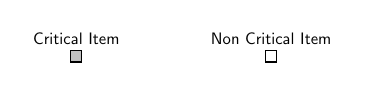
\begin{tikzpicture}[scale=0.6, every node/.style={scale=0.6}]
\node [label=Critical Item,draw,fill=gray!50] (node1) {};
\node [label={[name=l] Non Critical Item},draw,fill=white] (node2) at ([xshift=4cm]node1.east){};  
\end{tikzpicture}

				\caption{\label{fig:gant}Gantt Chart}
			\end{figure}
		\end{landscape}

		
		\bibliographystyle{plain}
		\bibliography{proposalbib}
	%	\printbibliography

\end{document}
